\documentclass[11pt]{article}
\usepackage[margin=1in]{geometry}
\usepackage{amsmath,amssymb,amsthm,mathtools,bm}
\usepackage{microtype}
\usepackage[T1]{fontenc}
\usepackage{lmodern}
\usepackage{booktabs,array,graphicx,enumitem}
\usepackage[hidelinks]{hyperref}
\setlist{nosep}
\newtheorem{theorem}{Theorem}[section]
\newtheorem{corollary}[theorem]{Corollary}
\newtheorem{lemma}[theorem]{Lemma}
\newtheorem{proposition}[theorem]{Proposition}
\theoremstyle{definition}
\newtheorem{definition}[theorem]{Definition}
\newtheorem{assumption}[theorem]{Assumption}
\theoremstyle{remark}
\newtheorem{remark}[theorem]{Remark}
\newtheorem{conjecture}{Conjecture}

\newcommand{\Qbar}{\overline{Q}}
\newcommand{\rhobar}{\overline{\rho}}
\newcommand{\dd}{\mathrm{d}}

\title{\textbf{Early-Universe Specialization of Hysterical Instability}\\[0.35em]
\large Cosmological closure, dust enhancement, and a timing route to rapid early galaxies}
\author{Andrew Bruce Boyd}
\date{Working mathematical formulation --- September 2026}

\begin{document}
\maketitle
\noindent\textit{Computational note.}
Proofs, exploratory experiments, and paper writing were assisted by generative AI.
Mathematical theorems stated in this paper are formally verified in Lean~4 in the
companion specifications, as faithful ports of the TeX arguments at the abstractions
recorded there, except results explicitly tagged as \emph{literature hypotheses}
(standard theorems cited from the literature and not re-proved here) or
\emph{physical inputs} (modeling assumptions outside mathematics).

\begin{abstract}
The response-theory paper already classifies closed-loop Hysterical Response by the spectral abscissa of the linearized gain Jacobian and supplies finite threshold times for nonzero unstable projections.
The present note does not re-prove that instability package.
It specializes it to a minimal post-decoupling cosmological model: a local response reservoir linearized to $\dot q+\gamma q=\sigma\delta$, closed attractively into dust growth.
Positive matter--response coupling makes the frozen Jacobian supercritical, so the inherited neutrality--instability theorem applies; a short comparison shows that at least one response-coupled root lies strictly above the ordinary pressureless-dust rate.
Interpreted physically, the same feedback is a candidate mechanism for \emph{rapid early galaxy formation}: small baryonic seeds can be amplified by a persistent response sector without importing a cold-dark-matter perturbative scaffold.
A Planck-like FLRW timing suite (nonlinear crossings, loss and delayed-activation scans, response amplification, and seed dependence) shows that a $10^{-5}$ baryon-only seed can reach nonlinear contrast by $z\simeq14$ for $\kappa\equiv\beta\sigma/H\gtrsim130$ when activated near recombination---compatible in timing with spectroscopically confirmed JWST galaxies at that epoch, but not a fit to their abundances or stellar masses.
A pressure extension and a conjectural capacity bridge complete the note.
\end{abstract}
\tableofcontents
\newpage

\section{Scope and status}
\label{sec:scope}
The response-theory paper~\cite{boyd2026response} proves the Hysterical Neutrality--Instability Theorem: if the closed-loop Jacobian $J$ has spectral abscissa $\alpha(J)>0$, neutrality is linearly unstable and every nonzero projection onto an unstable mode reaches any finite linear threshold in finite time, with delay only logarithmic in the seed~\cite{boyd2026response}.
Its ``how to apply'' recipe is explicit: name the physical variables, form the first-order Jacobian, and invoke the master theorem when $\alpha(J)>0$.

This paper follows that recipe for early structure and then asks the interpretive question the spectral facts invite: can the same instability operate fast enough, on an expanding background, to be relevant to the earliest observed galaxies?
It does \emph{not} re-derive exponential growth, amplitude-independent exponents, or threshold-time logarithms.
Those are inherited.
What is new is the cosmological closure, the dust-rate comparison, a pressured sufficient condition, a timing-viability benchmark against the JWST $z\sim14$ window, and the conjectural link to galactic capacity~\cite{boyd2026galactic}.

\begin{center}
\small
\begin{tabular}{@{}p{0.30\linewidth}p{0.62\linewidth}@{}}
\toprule
\textbf{Status} & \textbf{Ingredient}\\
\midrule
Inherited theorem & Neutrality--instability trichotomy; finite threshold time for nonzero unstable seeds~\cite{boyd2026response}.\\
Physical inputs & Local source--loss law; attractive gravitational closure; frozen / FLRW coefficient choices.\\
This paper & Jacobian identification; supercriticality; dust-rate enhancement; Jeans condition; full FLRW timing suite.\\
Interpretation & Candidate mechanism for rapid early galaxy formation (timing, not abundance).\\
Conjecture & Capacity-boundary crossing as early response-triggered assembly.\\
Deferred & CMB transfer functions, nonlinear hydrodynamics, stellar masses, luminosity functions.\\
\bottomrule
\end{tabular}
\end{center}

\section{Cosmological response closure}
\label{sec:closure}
\begin{assumption}[Local response source--loss law]
\label{ass:sourceloss}
A coarse-grained local response reservoir obeys
\begin{equation}
\dot Q+\Gamma Q=S(\rho,t),
\end{equation}
with $\Gamma\ge0$ and $S$ differentiable in density near a homogeneous background.
\end{assumption}

Writing $Q=\Qbar+\delta Q$, $\rho=\rhobar(1+\delta)$, and $q=\delta Q/\Qbar$ yields the linear response law
\begin{equation}
\label{eq:qlinear}
\boxed{\dot q+\gamma q=\sigma\delta,}
\end{equation}
with
\begin{equation}
\gamma\equiv\Gamma+\dot{\Qbar}/\Qbar,
\qquad
\sigma\equiv S_\rho(\rhobar,t)\rhobar/\Qbar.
\end{equation}

\begin{assumption}[Positive sourcing and nonnegative relaxation]
\label{ass:signs}
In the regime considered, $\sigma>0$ and $\gamma\ge0$.
\end{assumption}

\begin{assumption}[Linear attractive response closure]
\label{ass:closure}
At linear order,
\begin{equation}
\label{eq:deltamain}
\boxed{
\ddot\delta+2H\dot\delta=A(\delta+\beta q),
\qquad
A\equiv4\pi G\rhobar>0,\quad\beta>0.
}
\end{equation}
The dust growth equation without the $\beta q$ term is the standard Newtonian reduction (literature hypothesis; Remark~\ref{rem:dust}).
\end{assumption}

\begin{remark}[Dust growth equation]
\label{rem:dust}
Continuity plus Euler for pressureless matter in an expanding background reduce to $\ddot\delta+2H\dot\delta=A\delta$ when response feedback is absent; we do not re-derive that classical step.
\end{remark}

\section{Frozen Jacobian and inherited instability}
\label{sec:jacobian}
Freeze $H,A,\gamma,\sigma,\beta$ for a local spectral test and set $v=\dot\delta$.
The first-order state $(\delta,v,q)$ has Jacobian
\begin{equation}
\label{eq:J}
J=
\begin{pmatrix}
0&1&0\\
A&-2H&A\beta\\
\sigma&0&-\gamma
\end{pmatrix},
\end{equation}
with characteristic polynomial
\begin{equation}
\label{eq:poly}
P(\lambda)=(\lambda+\gamma)(\lambda^2+2H\lambda-A)-A\beta\sigma.
\end{equation}

\begin{lemma}[Supercritical offset]
\label{lem:P0}
Under Assumptions~\ref{ass:signs}--\ref{ass:closure} with $H\ge0$ and $A>0$,
\begin{equation}
P(0)=-A(\gamma+\beta\sigma)<0.
\end{equation}
\end{lemma}

\begin{proposition}[Cosmological instance of closed-loop instability]
\label{prop:instance}
Under the hypotheses of Lemma~\ref{lem:P0}, the frozen Jacobian~\eqref{eq:J} satisfies $\alpha(J)>0$.
The Hysterical Neutrality--Instability Theorem of the response-theory paper therefore applies~\cite{boyd2026response}: the homogeneous state is linearly unstable, and every nonzero unstable projection reaches any finite linear threshold in finite time with only logarithmic seed delay.
\end{proposition}

\begin{proof}
$P$ is a monic cubic with $P(0)<0$ and $P(\lambda)\to+\infty$ as $\lambda\to+\infty$, so it has a positive real root.
That root is an eigenvalue of $J$, hence $\alpha(J)>0$.
The instability and threshold-time statements are then exactly the Hysterical Neutrality--Instability Theorem and the finite-threshold-time corollary of~\cite{boyd2026response}; they are not re-proved here.
\end{proof}

\begin{remark}[What is not re-proved]
Amplitude-independent exponents, the logarithmic formula $t_*=\lambda_+^{-1}\log(X_*/|A_+|)$, and the stochastic excitation of an unstable mode without an imposed sign are already established in the response-theory paper.
This note only checks that the cosmological closure lands in the supercritical phase.
\end{remark}

\section{Enhancement over ordinary dust}
\label{sec:enhancement}
Without response coupling ($\beta\sigma=0$), the positive dust root is
\begin{equation}
\lambda_b=-H+\sqrt{H^2+A}>0.
\end{equation}

\begin{proposition}[Strict enhancement of the growing rate]
\label{prop:enhancement}
Under the hypotheses of Lemma~\ref{lem:P0}, there exists a real response-coupled root satisfying
\begin{equation}
\boxed{\lambda_+>\lambda_b.}
\end{equation}
\end{proposition}

\begin{proof}
$P(\lambda_b)=-A\beta\sigma<0$, while $P(\lambda)\to+\infty$ as $\lambda\to+\infty$, so continuity supplies a root strictly larger than $\lambda_b$.
\end{proof}

Positive response feedback therefore does more than recover the ordinary dust instability: it necessarily supplies a faster growing mode.

\section{Interpretation: rapid early galaxy formation}
\label{sec:interpretation}
The spectral facts above are mathematical.
Their intended physical reading in this paper is as a \emph{candidate mechanism for rapid early galaxy formation}.

In the standard picture, baryons fall into perturbations that have already grown in a cold-dark-matter sector.
Here the benchmark deliberately removes that perturbative CDM source and replaces it with a sourced memory field: small baryon fluctuations source $q$, which feeds back into gravity and accelerates $\delta$.
Proposition~\ref{prop:enhancement} is the linear reason the loop can outrun ordinary dust; the inherited threshold-time corollary is the reason arbitrarily small nonzero seeds remain viable on logarithmic clocks.

That reading is motivational until quantitative timing is checked.
Spectroscopically confirmed luminous galaxies already exist at $z\simeq14$, including JADES-GS-z14-0~\cite{Carniani2024}, placing assembled stellar systems only $\sim0.3\,\mathrm{Gyr}$ after the Big Bang in a Planck-like chronology~\cite{Planck2018}.
The next section asks only whether nonlinear \emph{matter contrast} can be reached by that epoch inside the effective model---not whether stellar masses, UV luminosity functions, or number densities are reproduced.

\section{Timing viability on an expanding background}
\label{sec:timing}
The experiments below restore the former early-universe timing suite: time-dependent FLRW coefficients, nonlinear-crossing times, loss and delayed-activation scans, response amplification, and seed dependence.
They answer a narrower question than a galaxy survey fit: can a primordial matter perturbation of order $10^{-5}$ become nonlinear by the epoch of the earliest spectroscopically confirmed JWST galaxies \emph{without} importing cold-dark-matter perturbations into the source term?

\subsection{Background and equations}
Restore a spatially flat Planck-like background~\cite{Planck2018}
\begin{equation}
H_0=67.4\,\mathrm{km\,s^{-1}\,Mpc^{-1}},\quad
\Omega_{m0}=0.315,\quad
\Omega_{b0}h^{2}=0.0224,\quad
\Omega_{r0}=9.2\times10^{-5},
\end{equation}
so $\Omega_{b0}\simeq0.0493$, and work in e-fold time $N=\ln a$.
Define the gravitationally weighted response $x\equiv\beta q$ and the dimensionless ratios
\begin{equation}
\label{eq:kappa-g}
\boxed{\kappa\equiv\frac{\beta\sigma}{H},\qquad g\equiv\frac{\gamma}{H}.}
\end{equation}
Holding $\kappa$ and $g$ constant is a phenomenological scaling assumption (source and loss track the Hubble rate).
The post-decoupling benchmark is
\begin{equation}
\label{eq:flrw}
\delta''+\Bigl(2+\frac{\dd\ln H}{\dd N}\Bigr)\delta'
=\frac32\,\Omega_b(a)\,(\delta+x),
\qquad
x'=\kappa\delta-gx,
\end{equation}
with primes $\dd/\dd N$.
Only the baryon fraction appears in the clustering term.
For comparison we also integrate a baryon-only curve (no $x$) and a standard total-matter clustering reference with $\tfrac32\Omega_m(a)\delta$ (not part of the Hysterical model).

\begin{remark}[Normalization]
The growth equations constrain $x=\beta q$.
A rescaling $q\mapsto cq$, $\beta\mapsto\beta/c$ leaves the gravitational dynamics invariant.
We use $\beta=1$ as the benchmark convention when plotting response amplitude; absolute claims about fractional $q$ require a microscopic normalization of $\beta$.
\end{remark}

\begin{assumption}[Fiducial timing experiment]
\label{ass:timing}
Integrate~\eqref{eq:flrw} from recombination $z_{\mathrm{on}}=1089$ with
$\delta_i=10^{-5}$, $\delta'_i=0$, $x_i=0$.
Define the nonlinear-crossing redshift $z_{\mathrm{nl}}$ by the first time $\delta=1$.
\end{assumption}

The choice $\delta'_i=0$ is conservative relative to seeding an already established growing mode.
The linear equations are not trusted beyond $\delta\sim1$; $z_{\mathrm{nl}}$ is an onset marker, not a collapse solution.
All quoted thresholds are regenerated by \texttt{run\_paper5\_timing.py}.

\subsection{Experiment I: nonlinearity by $z\simeq14$}
\begin{proposition}[Timing viability at $z\simeq14$]
\label{prop:timing}
In the benchmark of Assumption~\ref{ass:timing} with $g=0$, numerical integration of~\eqref{eq:flrw} yields
\begin{equation}
\boxed{\kappa_{\mathrm{crit}}(z_{\mathrm{nl}}=14,\,g=0)\simeq129.8.}
\end{equation}
Representative crossings are collected in Table~\ref{tab:znl-kappa}; Figure~\ref{fig:growth} shows the corresponding histories.
\end{proposition}

\begin{table}[ht]
\centering
\caption{Nonlinear-crossing redshift versus $\kappa$ for $g=0$, activation at $z_{\mathrm{on}}=1089$, and $\delta_i=10^{-5}$.}
\label{tab:znl-kappa}
\begin{tabular}{@{}rr@{}}
\toprule
$\kappa$ & $z_{\mathrm{nl}}$ \\
\midrule
50 & 1.91 \\
80 & 6.01 \\
100 & 9.12 \\
130 & 14.03 \\
150 & 17.38 \\
200 & 25.76 \\
300 & 41.80 \\
500 & 70.01 \\
\bottomrule
\end{tabular}
\end{table}

\begin{figure}[ht]
\centering
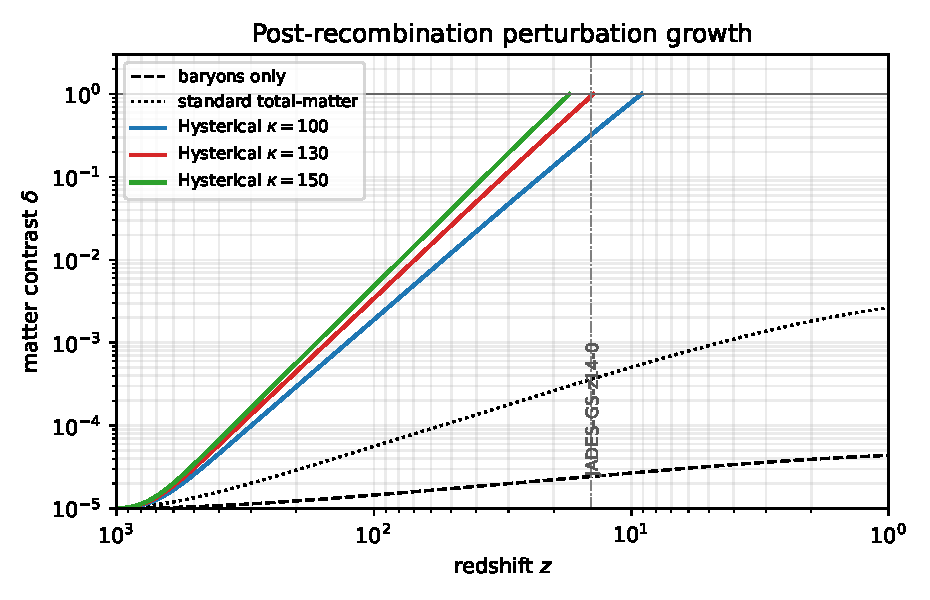
\includegraphics[width=0.88\textwidth]{paper5_growth_histories.pdf}
\caption{Matter-contrast evolution from recombination.
Baryon-only and standard total-matter curves are benchmarks.
In the Hysterical model, $\kappa=130$ is near the threshold for nonlinearity at $z\simeq14$, while $\kappa=150$ crosses earlier.
The vertical dash-dotted line marks the JADES-GS-z14-0 epoch~\cite{Carniani2024}.}
\label{fig:growth}
\end{figure}

The corresponding source timescale is of order $H/(\beta\sigma)\sim\kappa^{-1}$ Hubble times in this scaling convention; the required post-recombination response is therefore fast compared with cosmic expansion.

\subsection{Experiment II: finite response loss}
Loss competes directly with response accumulation.
For activation at $z=1089$, the minimum coupling required to reach $\delta=1$ by $z=14$ is
\begin{center}
\begin{tabular}{@{}rr@{}}
\toprule
$g=\gamma/H$ & $\kappa_{\mathrm{crit}}$ \\
\midrule
0 & 129.8 \\
0.3 & 142.2 \\
1 & 171.1 \\
3 & 254.1 \\
\bottomrule
\end{tabular}
\end{center}
Long response memory is cosmologically valuable, but nonzero loss does not remove the instability; it raises the required source strength.
This is the expanding-background realization of the frozen-coefficient intuition from Sections~\ref{sec:jacobian}--\ref{sec:enhancement}.

\subsection{Experiment III: delayed activation after recombination}
A central cosmological concern is the CMB.
If the Hysterical perturbation were already strongly active in the tightly coupled photon--baryon plasma, it could modify the acoustic transfer function.
We therefore repeat the experiment with the perturbative response switched on only at a chosen $z_{\mathrm{on}}<1089$.

\begin{figure}[ht]
\centering
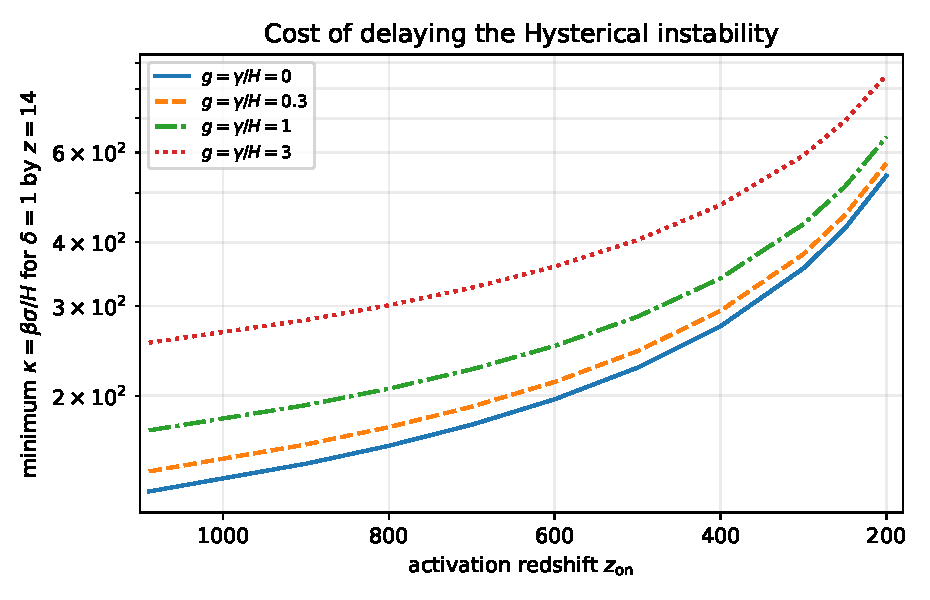
\includegraphics[width=0.88\textwidth]{paper5_activation_cost.pdf}
\caption{Minimum $\kappa$ required for a $10^{-5}$ seed to reach $\delta=1$ by $z=14$, as a function of turn-on redshift, for several loss parameters $g$.
Delaying activation leaves less logarithmic expansion time and therefore demands a stronger source.}
\label{fig:activation}
\end{figure}

For $g=0$,
\begin{equation}
\kappa_{\mathrm{crit}}\simeq
\begin{cases}
130, & z_{\mathrm{on}}=1089,\\
197, & z_{\mathrm{on}}=600,\\
274, & z_{\mathrm{on}}=400,\\
356, & z_{\mathrm{on}}=300,\\
540, & z_{\mathrm{on}}=200.
\end{cases}
\end{equation}
A post-recombination or delayed Hysterical instability remains mathematically capable of producing very early nonlinearity.
This does not prove CMB compatibility; it shows that suppressing pre-recombination perturbative response does not automatically remove the early-growth mechanism.

\subsection{Experiment IV: amplification of the response perturbation}
\begin{figure}[ht]
\centering
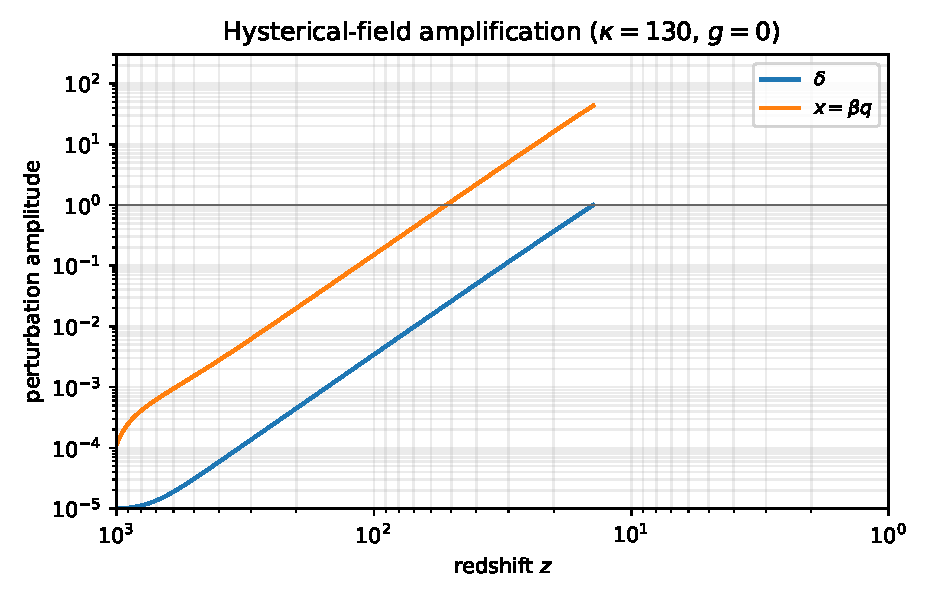
\includegraphics[width=0.88\textwidth]{paper5_amplification.pdf}
\caption{Amplification of matter and the gravitationally weighted response for $\kappa=130$, $g=0$.
In the benchmark normalization $\beta=1$, $x$ may also be read as the fractional response perturbation $q$.
Once either variable is order unity a nonlinear treatment is required.}
\label{fig:amp}
\end{figure}

For the near-critical $\kappa=130$, $g=0$ benchmark, $x=\beta q$ grows earlier and faster in amplitude than $\delta$ because it is directly sourced by the accumulated matter perturbation.
This is the expanding-background counterpart of the dynamical susceptibility of the frozen analysis.
The invariant statement is about $x$; with $\beta=1$ the same plot may be read as $q$.

\subsection{Experiment V: arbitrarily small seeds}
The inherited threshold-time corollary already implies that the unstable exponent does not depend on seed amplitude.
The expanding-background experiment shows the corresponding timing effect at fixed $\kappa=150$, $g=0$:
\begin{center}
\begin{tabular}{@{}rr@{}}
\toprule
$\delta_i$ & $z_{\mathrm{nl}}$ \\
\midrule
$10^{-3}$ & 79.0 \\
$10^{-4}$ & 37.3 \\
$10^{-5}$ & 17.4 \\
$10^{-6}$ & 7.82 \\
$10^{-7}$ & 3.22 \\
$10^{-8}$ & 0.96 \\
\bottomrule
\end{tabular}
\end{center}

\begin{figure}[ht]
\centering
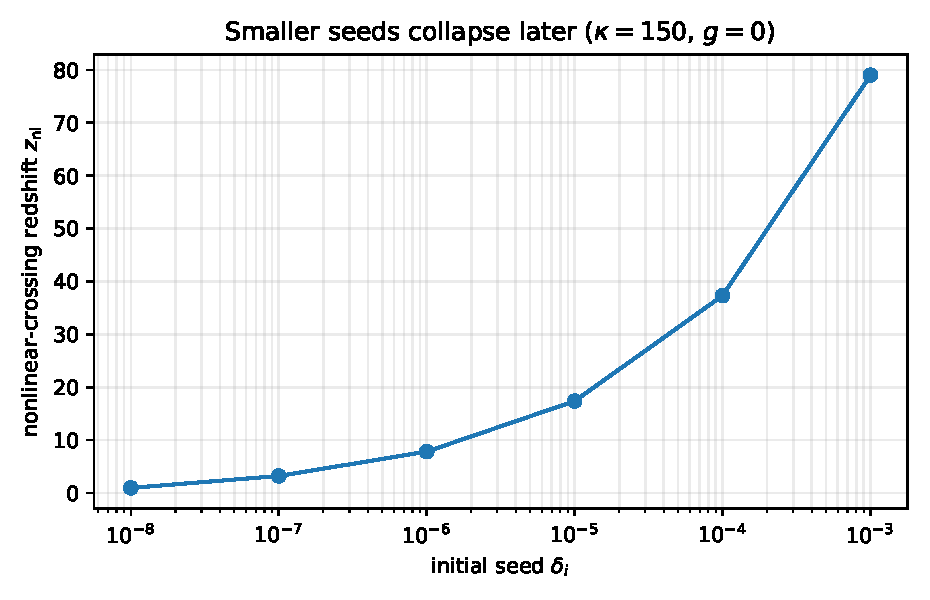
\includegraphics[width=0.88\textwidth]{paper5_seed_dependence.pdf}
\caption{Nonlinear-crossing redshift versus seed amplitude at fixed $\kappa=150$, $g=0$.
Arbitrarily smaller nonzero seeds remain unstable but cross later.}
\label{fig:seeds}
\end{figure}

The seed does not acquire a smaller growth exponent as its amplitude tends to zero; it simply takes longer to cross the chosen nonlinear threshold.

\subsection{JWST timing and the $\Lambda$CDM contrast}
JWST has spectroscopically confirmed luminous systems at $z\simeq14$, including JADES-GS-z14-0 at $z=14.32^{+0.08}_{-0.20}$~\cite{Carniani2024}, corresponding to roughly $0.3\,\mathrm{Gyr}$ after the Big Bang in the adopted background.
The present calculation addresses only whether gravitational matter contrast can enter a nonlinear regime by such epochs.
It does not map $\delta=1$ to a stellar mass, luminosity, or number density.
The correct conclusion is therefore that the model can match the timing requirement for $z\sim14$ nonlinearity in a finite parameter region.
It would be premature to claim a fit to the JWST population.

Mechanistically, standard $\Lambda$CDM grows baryons in a pre-existing cold-dark-matter scaffold.
Here that perturbative CDM source is removed and replaced by a sourced memory field:
\[
\begin{aligned}
&\text{small baryon fluctuation}
\longrightarrow
\text{Hysterical perturbation}\\
&\qquad\longrightarrow
\text{additional gravity}
\longrightarrow
\text{larger baryon fluctuation.}
\end{aligned}
\]
The Hysterical mechanism can compensate for the missing perturbative scaffold if $\kappa$ is sufficiently large and $g$ sufficiently small.
The difference becomes observational only after a complete transfer function and abundance calculation are supplied.

\begin{remark}[Status of the timing experiments]
\label{rem:timing-status}
Proposition~\ref{prop:timing} and Tables/Figures in this section are reproducible numerical experiments in a disclosed effective model, not Lean-checked theorems.
They establish \emph{timing possibility} and map the $(\kappa,g,z_{\mathrm{on}},\delta_i)$ dependence.
They do not fix a microscopic $\kappa$, prove CMB safety, or fit JWST abundances.
\end{remark}

\subsection{Open gaps retained from the timing suite}
\begin{enumerate}[label=(\arabic*)]
\item Microscopic normalization of $\kappa=\beta\sigma/H$ and $g=\gamma/H$ from the underlying open-system dynamics.
\item Joint pre-recombination evolution of photons, baryons, metric perturbations, and the response field.
\item Homogeneous Friedmann closure if the response is to replace dark matter in the background as well as in perturbations.
\item Scale dependence from propagation, pressure, finite memory length, or relativistic closure.
\item Nonlinear collapse, cooling, star formation, and the galactic capacity condition beyond $\delta=1$.
\item Abundance predictions $n(M_\star,z)$ or the UV luminosity function.
\end{enumerate}

\section{Pressure extension}
\label{sec:jeans}
With a Fourier pressure term $B_k=c_s^2k^2/a^2\ge0$, the frozen characteristic polynomial becomes
\begin{equation}
P_k(\lambda)=(\lambda+\gamma)(\lambda^2+2H\lambda+B_k-A)-A\beta\sigma.
\end{equation}

\begin{proposition}[Sufficient response-induced Jeans crossing]
\label{prop:jeans}
If $A\beta\sigma>\gamma(B_k-A)$, then $P_k(0)<0$, so $P_k$ has a positive real root and $\alpha>0$ for the pressured frozen system.
\end{proposition}

Pre-recombination photon--baryon physics is outside the present scope; the proposition is only the algebraic sufficient condition once a pressured dust model is assumed.

\section{Capacity bridge}
\label{sec:bridge}
Galactic modelling conjectures a formation/retention capacity boundary $Q\gtrsim O(\sqrt{M_b})$~\cite{boyd2026galactic}.
Linear instability and timing viability amplify $\delta Q$ on a cosmologically interesting clock; they do not by themselves prove that a proto-galactic region crosses that boundary before ordinary baryonic growth would.

\begin{conjecture}[Early response-triggered assembly]
\label{conj:assembly}
In a post-decoupling proto-galactic region with sufficiently large $\sigma$ and sufficiently persistent response, the inherited unstable mode drives local $Q$ fluctuations across the response-capacity boundary before ordinary baryonic growth reaches the same nonlinear state.
\end{conjecture}

\section{Logical status of the results}
\label{sec:status}
\begin{center}
\small
\begin{tabular}{@{}p{0.42\linewidth}p{0.50\linewidth}@{}}
\toprule
\textbf{Quantity / claim} & \textbf{Status}\\
\midrule
Master instability / threshold time & Inherited from~\cite{boyd2026response} (Lean there).\\
Source--loss law and attractive closure & Physical inputs.\\
Dust growth equation without response & Literature hypothesis (Remark~\ref{rem:dust}).\\
Frozen characteristic polynomial $P(\lambda)$ & Definition (Lean).\\
$P(0)<0$ under positive coupling & Lemma~\ref{lem:P0} (Lean).\\
$\alpha(J)>0$ via positive root of $P$ & Proposition~\ref{prop:instance} (Lean positive-root step; master theorem inherited).\\
Dust-rate enhancement & Proposition~\ref{prop:enhancement} (Lean).\\
Rapid early-galaxy interpretation & Physical reading of the spectral facts (Sec.~\ref{sec:interpretation}).\\
FLRW timing suite (I--V) & Numerical experiments (Sec.~\ref{sec:timing}; not Lean).\\
JWST $z\sim14$ epoch & Observational timing target~\cite{Carniani2024}.\\
Jeans-sufficient condition & Proposition~\ref{prop:jeans} (Lean).\\
Capacity-bridge assembly & Conjecture~\ref{conj:assembly}.\\
Abundances / stellar masses / CMB transfer & Deferred (open gaps in Sec.~\ref{sec:timing}).\\
\bottomrule
\end{tabular}
\end{center}

\section{Conclusion}
\label{sec:conclusion}
Once a local response reservoir is sourced by matter and closed attractively into post-decoupling dust growth, the frozen linear system is supercritical under positive coupling.
Everything that follows for exponential growth and arbitrarily small nonzero seeds is already in the response-theory instability package.
The cosmological specialization adds dust-rate enhancement, a pressured sufficient condition, and the former early-universe timing suite: in a Planck-like baryon-only FLRW benchmark, nonlinear contrast by $z\simeq14$ is reachable for $\kappa\gtrsim130$ at low loss, with mapped costs for finite loss, delayed activation, and smaller seeds.
That suite is the quantitative justification for reading the instability as a candidate mechanism for rapid early galaxy formation: it can meet the JWST timing window without a CDM perturbative scaffold.
It is not yet a prediction of galaxy abundances, stellar masses, or CMB-safe parameters; those remain the next calculations.

\bibliographystyle{plain}
\bibliography{paper_5_refs}
\end{document}
